

\section{OpticalElement: \textquotedbl{}micado\_sci\_detector\textquotedbl{}%
  \label{opticalelement-micado-sci-detector}%
}

\textbf{Element}: detector

\textbf{Alias}: DET

\textbf{Description}: List of MICADO detector effects relevant for astronomers


\subsection{Global properties%
  \label{global-properties}%
}

\begin{quote}
\begin{alltt}
\begin{lstlisting}[frame=single]
image_plane_id : 0
   temperature : -230
           dit : !OBS.dit
          ndit : !OBS.ndit
         width : 4096
        height : 4096
             x : 0
             y : 0
  element_name : micado_sci_detector
\end{lstlisting}
\end{alltt}
\end{quote}


\subsection{Effects%
  \label{effects}%
}

Summary of Effects included in this optical element:

\setlength{\DUtablewidth}{\linewidth}
\begin{longtable*}[c]{|p{0.195\DUtablewidth}|p{0.233\DUtablewidth}|p{0.242\DUtablewidth}|p{0.090\DUtablewidth}|p{0.195\DUtablewidth}|}
\hline
\textbf{%
element
} & \textbf{%
name
} & \textbf{%
class
} & \textbf{%
included
} & \textbf{%
z\_orders
} \\
\hline
\endfirsthead
\hline
\textbf{%
element
} & \textbf{%
name
} & \textbf{%
class
} & \textbf{%
included
} & \textbf{%
z\_orders
} \\
\hline
\endhead
\multicolumn{5}{c}{\hfill ... continued on next page} \\
\endfoot
\endlastfoot

micado\_sci\_detector
 & 
micado\_detector\_window
 & 
DetectorWindow
 & 
True
 & 
{[}90, 290, 390, 490{]}
 \\
\hline

micado\_sci\_detector
 & 
h4rg\_qe\_curve
 & 
QuantumEfficiencyCurve
 & 
True
 & 
{[}113, 513{]}
 \\
\hline

micado\_sci\_detector
 & 
exposure\_action
 & 
SummedExposure
 & 
True
 & 
{[}860{]}
 \\
\hline

micado\_sci\_detector
 & 
dark\_current
 & 
DarkCurrent
 & 
True
 & 
{[}830{]}
 \\
\hline

micado\_sci\_detector
 & 
shot\_noise
 & 
ShotNoise
 & 
True
 & 
{[}820{]}
 \\
\hline

micado\_sci\_detector
 & 
h4rg\_detector\_linearity
 & 
LinearityCurve
 & 
False
 & 
{[}840{]}
 \\
\hline

micado\_sci\_detector
 & 
readout\_noise
 & 
PoorMansHxRGReadoutNoise
 & 
True
 & 
{[}811{]}
 \\
\hline
\end{longtable*}
\label{tbl-micado-sci-detector}


\subsubsection{DetectorWindow: \textquotedbl{}micado\_detector\_window\textquotedbl{}%
  \label{detectorwindow-micado-detector-window}%
}

\textbf{Included by default}: \texttt{True}

\textbf{File Description}:

\textbf{Class Description}: For when a full DetectorList if too cumbersome

\textbf{Changes}:

\begin{itemize}
\item \end{itemize}


\paragraph{Data%
  \label{data}%
}

\begin{figure}[H]
\noindent\makebox[\linewidth][c]{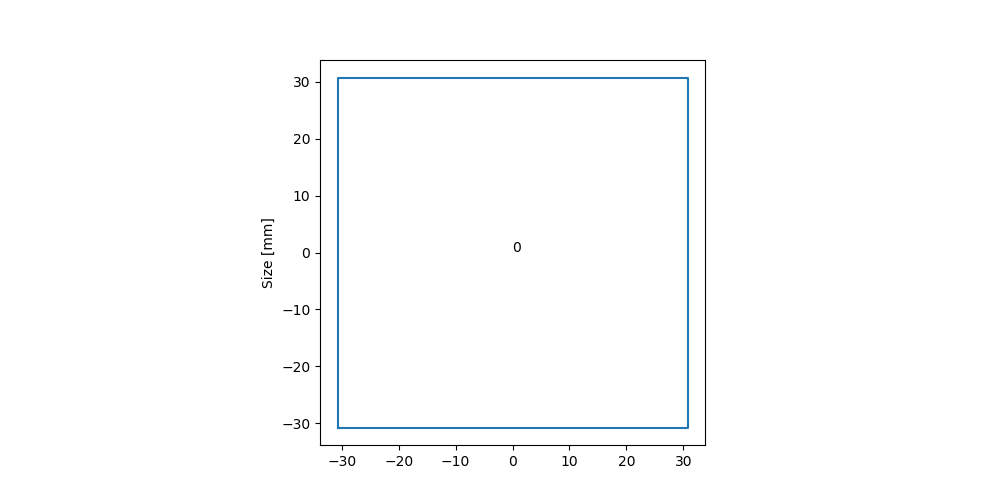
\includegraphics{micado_detector_window.png}}\phantomsection\label{fig-micado-detector-window}
\end{figure}

\setlength{\DUtablewidth}{\linewidth}
\begin{longtable*}[c]{|p{0.051\DUtablewidth}|p{0.086\DUtablewidth}|p{0.086\DUtablewidth}|p{0.133\DUtablewidth}|p{0.145\DUtablewidth}|p{0.075\DUtablewidth}|p{0.063\DUtablewidth}|p{0.133\DUtablewidth}|}
\hline
\textbf{%
id
} & \textbf{%
x\_cen
} & \textbf{%
y\_cen
} & \textbf{%
x\_size
} & \textbf{%
y\_size
} & \textbf{%
angle
} & \textbf{%
gain
} & \textbf{%
pixel\_size
} \\
\hline
\endfirsthead
\hline
\textbf{%
id
} & \textbf{%
x\_cen
} & \textbf{%
y\_cen
} & \textbf{%
x\_size
} & \textbf{%
y\_size
} & \textbf{%
angle
} & \textbf{%
gain
} & \textbf{%
pixel\_size
} \\
\hline
\endhead
\multicolumn{8}{c}{\hfill ... continued on next page} \\
\endfoot
\endlastfoot

0
 & 
!DET.x
 & 
!DET.y
 & 
!DET.width
 & 
!DET.height
 & 
0
 & 
1
 & 
0.015
 \\
\hline
\end{longtable*}
\label{tbl-micado-detector-window}


\paragraph{Meta-data%
  \label{meta-data}%
}

\begin{quote}
\begin{alltt}
\begin{lstlisting}[frame=single]
            filename : None
                name : micado_detector_window
          orig_units : pixel
          x_cen_unit : pixel
          y_cen_unit : pixel
         x_size_unit : pixel
         y_size_unit : pixel
     pixel_size_unit : mm
          angle_unit : deg
           gain_unit : electron/adu
      image_plane_id : 0
         temperature : -230
                 dit : !OBS.dit
                ndit : !OBS.ndit
        element_name : micado_sci_detector
             z_order : [90, 290, 390, 490]
             include : True
         pixel_scale : !INST.pixel_scale
    active_detectors : all
 report_plot_include : True
report_table_include : True
\end{lstlisting}
\end{alltt}
\end{quote}


\subsubsection{QuantumEfficiencyCurve: \textquotedbl{}h4rg\_qe\_curve\textquotedbl{}%
  \label{quantumefficiencycurve-h4rg-qe-curve}%
}

\textbf{Included by default}: \texttt{True}

\textbf{File Description}: Quantum efficiency curves for each detector

\textbf{Class Description}: <no docstring>

\textbf{Changes}:

\begin{itemize}
\item 2018-11-19 (KL) updated meta data to new format

\item 2019-08-09 (KL) Added action keyword to meta data
\end{itemize}


\paragraph{Data%
  \label{id1}%
}

\begin{figure}[H]
\noindent\makebox[\linewidth][c]{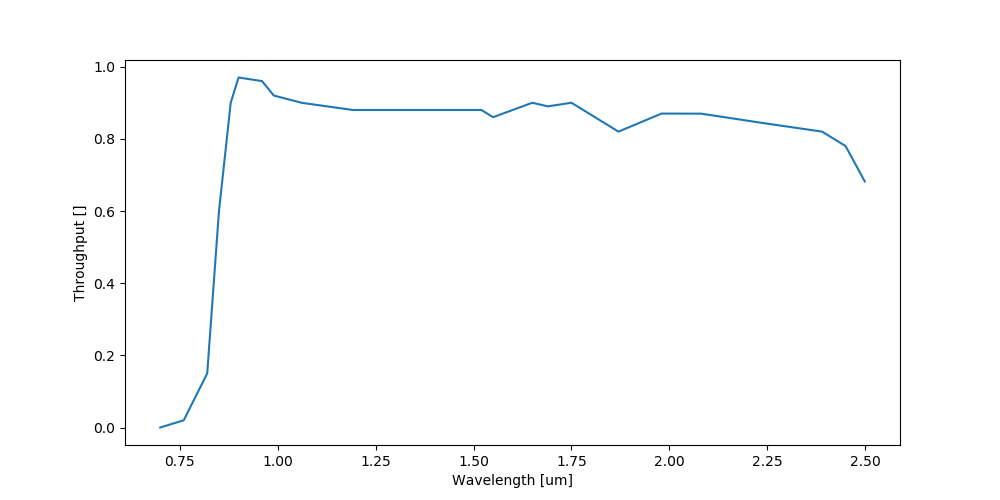
\includegraphics{h4rg_qe_curve.png}}\phantomsection\label{fig-h4rg-qe-curve}
\end{figure}


\paragraph{Meta-data%
  \label{id2}%
}

\begin{quote}
\begin{alltt}
\begin{lstlisting}[frame=single]
            filename : QE_detector_H2RG.dat
                name : h4rg_qe_curve
      image_plane_id : 0
         temperature : -230
                 dit : 60
                ndit : 1
               width : 4096
              height : 4096
                   x : 0
                   y : 0
        element_name : micado_sci_detector
              author : Kieran Leschinski
             sources : Finger+ 2008 SPIE
        date_created : 2016-01-01
       date_modified : 2019-08-09
                type : detector:quantum_efficiency
              status : Design, guestimated by reading off the graph in Finger+ 2008
     wavelength_unit : um
              action : transmission
             z_order : [113, 513]
             include : True
        ignore_wings : False
            wave_min : 0.7
            wave_max : 2.5
           wave_unit : um
            wave_bin : 0.001
 report_plot_include : True
report_table_include : False
            position : -1
\end{lstlisting}
\end{alltt}
\end{quote}


\subsubsection{SummedExposure: \textquotedbl{}exposure\_action\textquotedbl{}%
  \label{summedexposure-exposure-action}%
}

\textbf{Included by default}: \texttt{True}

\textbf{File Description}: Summing up sky signal for all DITs and NDITs

\textbf{Class Description}: Simulates a summed stack of \texttt{ndit} exposures

\textbf{Changes}:

\begin{itemize}
\item \end{itemize}


\paragraph{Data%
  \label{id3}%
}


\paragraph{Meta-data%
  \label{id4}%
}

\begin{quote}
\begin{alltt}
\begin{lstlisting}[frame=single]
      filename : None
          name : exposure_action
image_plane_id : 0
   temperature : -230
           dit : !OBS.dit
          ndit : !OBS.ndit
         width : 4096
        height : 4096
             x : 0
             y : 0
  element_name : micado_sci_detector
       z_order : [860]
       include : True
\end{lstlisting}
\end{alltt}
\end{quote}


\subsubsection{DarkCurrent: \textquotedbl{}dark\_current\textquotedbl{}%
  \label{darkcurrent-dark-current}%
}

\textbf{Included by default}: \texttt{True}

\textbf{File Description}: MICADO dark current

\textbf{Class Description}: required: dit, ndit, value

\textbf{Changes}:

\begin{itemize}
\item \end{itemize}


\paragraph{Data%
  \label{id5}%
}


\paragraph{Meta-data%
  \label{id6}%
}

\begin{quote}
\begin{alltt}
\begin{lstlisting}[frame=single]
      filename : None
          name : dark_current
image_plane_id : 0
   temperature : -230
           dit : !OBS.dit
          ndit : !OBS.ndit
         width : 4096
        height : 4096
             x : 0
             y : 0
  element_name : micado_sci_detector
         value : 0.1
       z_order : [830]
       include : True
\end{lstlisting}
\end{alltt}
\end{quote}


\subsubsection{ShotNoise: \textquotedbl{}shot\_noise\textquotedbl{}%
  \label{shotnoise-shot-noise}%
}

\textbf{Included by default}: \texttt{True}

\textbf{File Description}: apply poisson shot noise to images

\textbf{Class Description}: <no docstring>

\textbf{Changes}:

\begin{itemize}
\item \end{itemize}


\paragraph{Data%
  \label{id7}%
}


\paragraph{Meta-data%
  \label{id8}%
}

\begin{quote}
\begin{alltt}
\begin{lstlisting}[frame=single]
      filename : None
          name : shot_noise
image_plane_id : 0
   temperature : -230
           dit : !OBS.dit
          ndit : !OBS.ndit
         width : 4096
        height : 4096
             x : 0
             y : 0
  element_name : micado_sci_detector
       z_order : [820]
       include : True
   random_seed : !SIM.random.seed
\end{lstlisting}
\end{alltt}
\end{quote}


\subsubsection{LinearityCurve: \textquotedbl{}h4rg\_detector\_linearity\textquotedbl{}%
  \label{linearitycurve-h4rg-detector-linearity}%
}

\textbf{Included by default}: \texttt{False}

\textbf{File Description}: Linearity characteristics of H4RG chips

\textbf{Class Description}: <no docstring>

\textbf{Changes}:

\begin{itemize}
\item 2018-11-19 (KL) updated meta data to new format

\item 2019-08-14 (KL) replaced long 1000000000 with 1e99
\end{itemize}


\paragraph{Data%
  \label{id9}%
}

\begin{figure}[H]
\noindent\makebox[\linewidth][c]{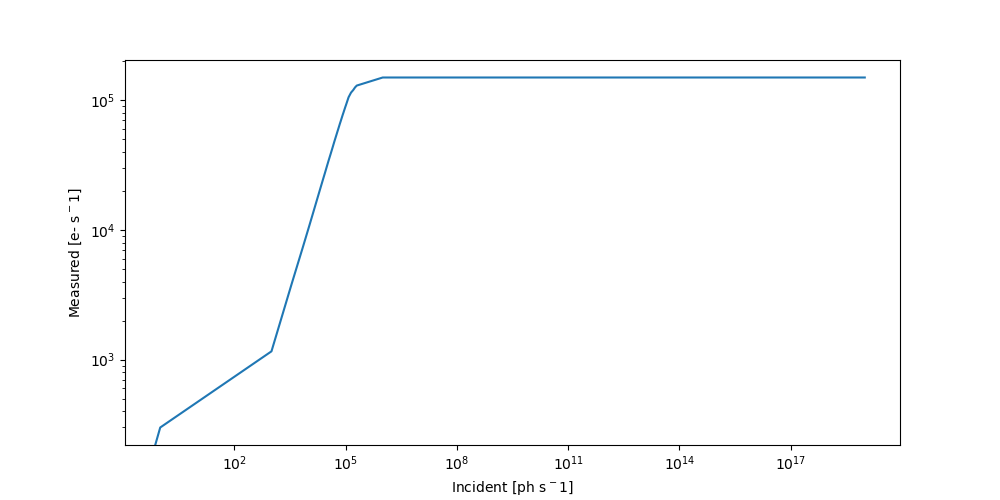
\includegraphics{h4rg_detector_linearity.png}}\phantomsection\label{fig-h4rg-detector-linearity}
\end{figure}


\paragraph{Meta-data%
  \label{id10}%
}

\begin{quote}
\begin{alltt}
\begin{lstlisting}[frame=single]
            filename : FPA_linearity.dat
                name : h4rg_detector_linearity
             include : False
      image_plane_id : 0
         temperature : -230
                 dit : !OBS.dit
                ndit : !OBS.ndit
               width : 4096
              height : 4096
                   x : 0
                   y : 0
        element_name : micado_sci_detector
              author : Kieran Leschinski
             sources : Ingraham+ 2014 - Gemini Calibrations II for H2RG
        date_created : 2016-01-01
       date_modified : 2018-11-19
                type : detector:linearity
              status : Design, approximated from the H2RG
       incident_unit : ph
       measured_unit : ph
             z_order : [840]
 report_plot_include : True
report_table_include : False
\end{lstlisting}
\end{alltt}
\end{quote}


\subsubsection{PoorMansHxRGReadoutNoise: \textquotedbl{}readout\_noise\textquotedbl{}%
  \label{poormanshxrgreadoutnoise-readout-noise}%
}

\textbf{Included by default}: \texttt{True}

\textbf{File Description}: Readout noise frames

\textbf{Class Description}: <no docstring>

\textbf{Changes}:

\begin{itemize}
\item \end{itemize}


\paragraph{Data%
  \label{id11}%
}


\paragraph{Meta-data%
  \label{id12}%
}

\begin{quote}
\begin{alltt}
\begin{lstlisting}[frame=single]
            filename : None
                name : readout_noise
      image_plane_id : 0
         temperature : -230
                 dit : !OBS.dit
                ndit : !OBS.ndit
               width : 4096
              height : 4096
                   x : 0
                   y : 0
        element_name : micado_sci_detector
           noise_std : 12
          n_channels : 64
             z_order : [811]
             include : True
   pedestal_fraction : 0.3
       read_fraction : 0.4
       line_fraction : 0.25
    channel_fraction : 0.05
         random_seed : !SIM.random.seed
 report_plot_include : False
report_table_include : False
\end{lstlisting}
\end{alltt}
\end{quote}
